In this chapter, we define label prediction methods and show how they can
be applied on graphs. We present different problems we can solve using
label prediction methods and how we can incorporate graph metrics, such as
the diffusion state distance (DSD), into these methods. We use the terms
label prediction methods and vertex classifiers interchangeably.

\section{Problem Definition}
\label{sec:label_prediction_methods}
We begin by presenting definitions relating to labels of graphs.

\begin{definition}
A \textbf{partially labeled graph} is a graph $G$ and a function
$c : V_{G_p} \to S$, where $S$ is an arbitrary set of labels, and
$V_{G_p} \subseteq V_G$ with
$|V_{G_p}| = \left\lfloor{p \cdot |V_G|}\right\rfloor$, $0 \leq p \leq 1$.

The set $V_G \setminus V_{G_p}$ is called the set of \textbf{unlabeled} 
vertices of $G$.

The function $c$ is called a \textbf{partial labeling} of $G$.
\end{definition}

\begin{definition}
A \textbf{censoring} of a labeled graph $G$ and its labeling function
$c : V_G \to S$ is a set $V_{G_c}$ and a function
$c_p: V_G \setminus V_{G_c} \to S$ such that $c_p$ is a partial labeling
of $G$.

The function $c$ of the labeled graph $G$ is called the \textbf{ground truth labeling} of the
censoring of $G$. Note that the set $V_{G_c}$ is the set of unlabeled vertices of the partial
labeling of $G$.
\end{definition}

Given a partially labeled graph $G$, a censoring $(V_{G_c}, c_{censor})$
of $G$, and a ground truth labeling $c_{gt}$ of $G$, a 
\textbf{label prediction method} is an algorithm that attempts to correctly 
guess the labels of the unlabeled vertices $V_{G_c}$ with respect to the
ground truth labels $c_{gt}(v), v \in V_{G_c}$.

In order for a label prediction method on a graph to have any success, the ground truth labeling
must reflect some underlying graph structure. If the labels in a graph were assigned at random to
each vertex, a label prediction algorithm could not be expected to perform better than randomly
guessing the labels on vertices.

We now discuss label prediction methods that we considered for our 
simulations in Chapter 6.

% Fix wording make more mathematical
\subsection{Majority Voting Algorithm}
Cao, Zhang, Park, Daniels, Crovella, Cowen, and Hescott~\cite{10.1371/journal.pone.0076339}
describe a simple prediction method called the neighborhood majority voting
algorithm. This algorithm considers each vertex with unknown label and has
its neighbors vote on the label for the vertex. We considered two
implementations of this algorithm, which differ in how they determine which neighbors vote. One 
implementation considers each vertex $v \in V$ and all neighbors of $v$ within an $\varepsilon$
distance from $v$ (a ball of radius $\varepsilon$). The $\varepsilon$ distance depends on the metric
under consideration, and may be changed as a parameter. In an unweighted scheme, each neighbor
within the ball of radius $\varepsilon$ votes equally for their own label. In 
a weighted scheme, we must consider a metric on a graph to use (chapter 4).
Using this metric, each neighbor gets a vote proportional to the reciprocal 
of its distance to the vertex $v$ in
consideration. The other implementation of this algorithm considers each vertex $v \in V$ and
the $k$-nearest neighbors of $v$ with respect to the graph metric. Voting is done similarly in both an unweighted and weighted
scheme.

There are other prediction methods that exist, such as the $\chi^{2}$ neighborhood algorithm, the
multi-way cut algorithm, and the functional flow algorithm~\cite{10.1371/journal.pone.0076339}.
These prediction methods can also be modified to incorporate graph metrics discussed in chapter 4.
However, we only consider the weighted majority voting algorithm for our simulations in order to
keep the intuition behind results of this algorithm simple.

\section{Real World Data}

In this section, we discuss three different examples of graph-based studies performed on real world
data. We discuss how these examples constructed graphs from their data, and what kind of studies
were performed on the resulting graphs. These studies give constructions of different graph
representations of data that we can use to test the effects of different metrics with prediction
algorithms.

\subsection{Protein-Protein Interaction (PPI) networks}
Cao et al.~\cite{10.1371/journal.pone.0076339} studied the prediction of protein
functional labels on the \emph{S. cerevisiae} protein-protein interaction (PPI) network. The
authors constructed a graph using annotated physical interactions in this PPI network. Proteins
corresponded to vertices, and an annotated physical interaction between two proteins corresponded to
an edge. Cao et al. removed redundant edges and the largest connected component was selected,
resulting in a graph of 4990 vertices and 74,310 edges. They also noted that PPI networks are known
to resemble small-world networks, as they have a small maximum shortest path, and a small
characteristic path length. This implies that most vertices in the graph are close to every other
vertex in the graph. Figure \ref{fig:PPI_example} shows an example of functional annotation using
the DSD from Cao et al.

\begin{figure}[h] \centering 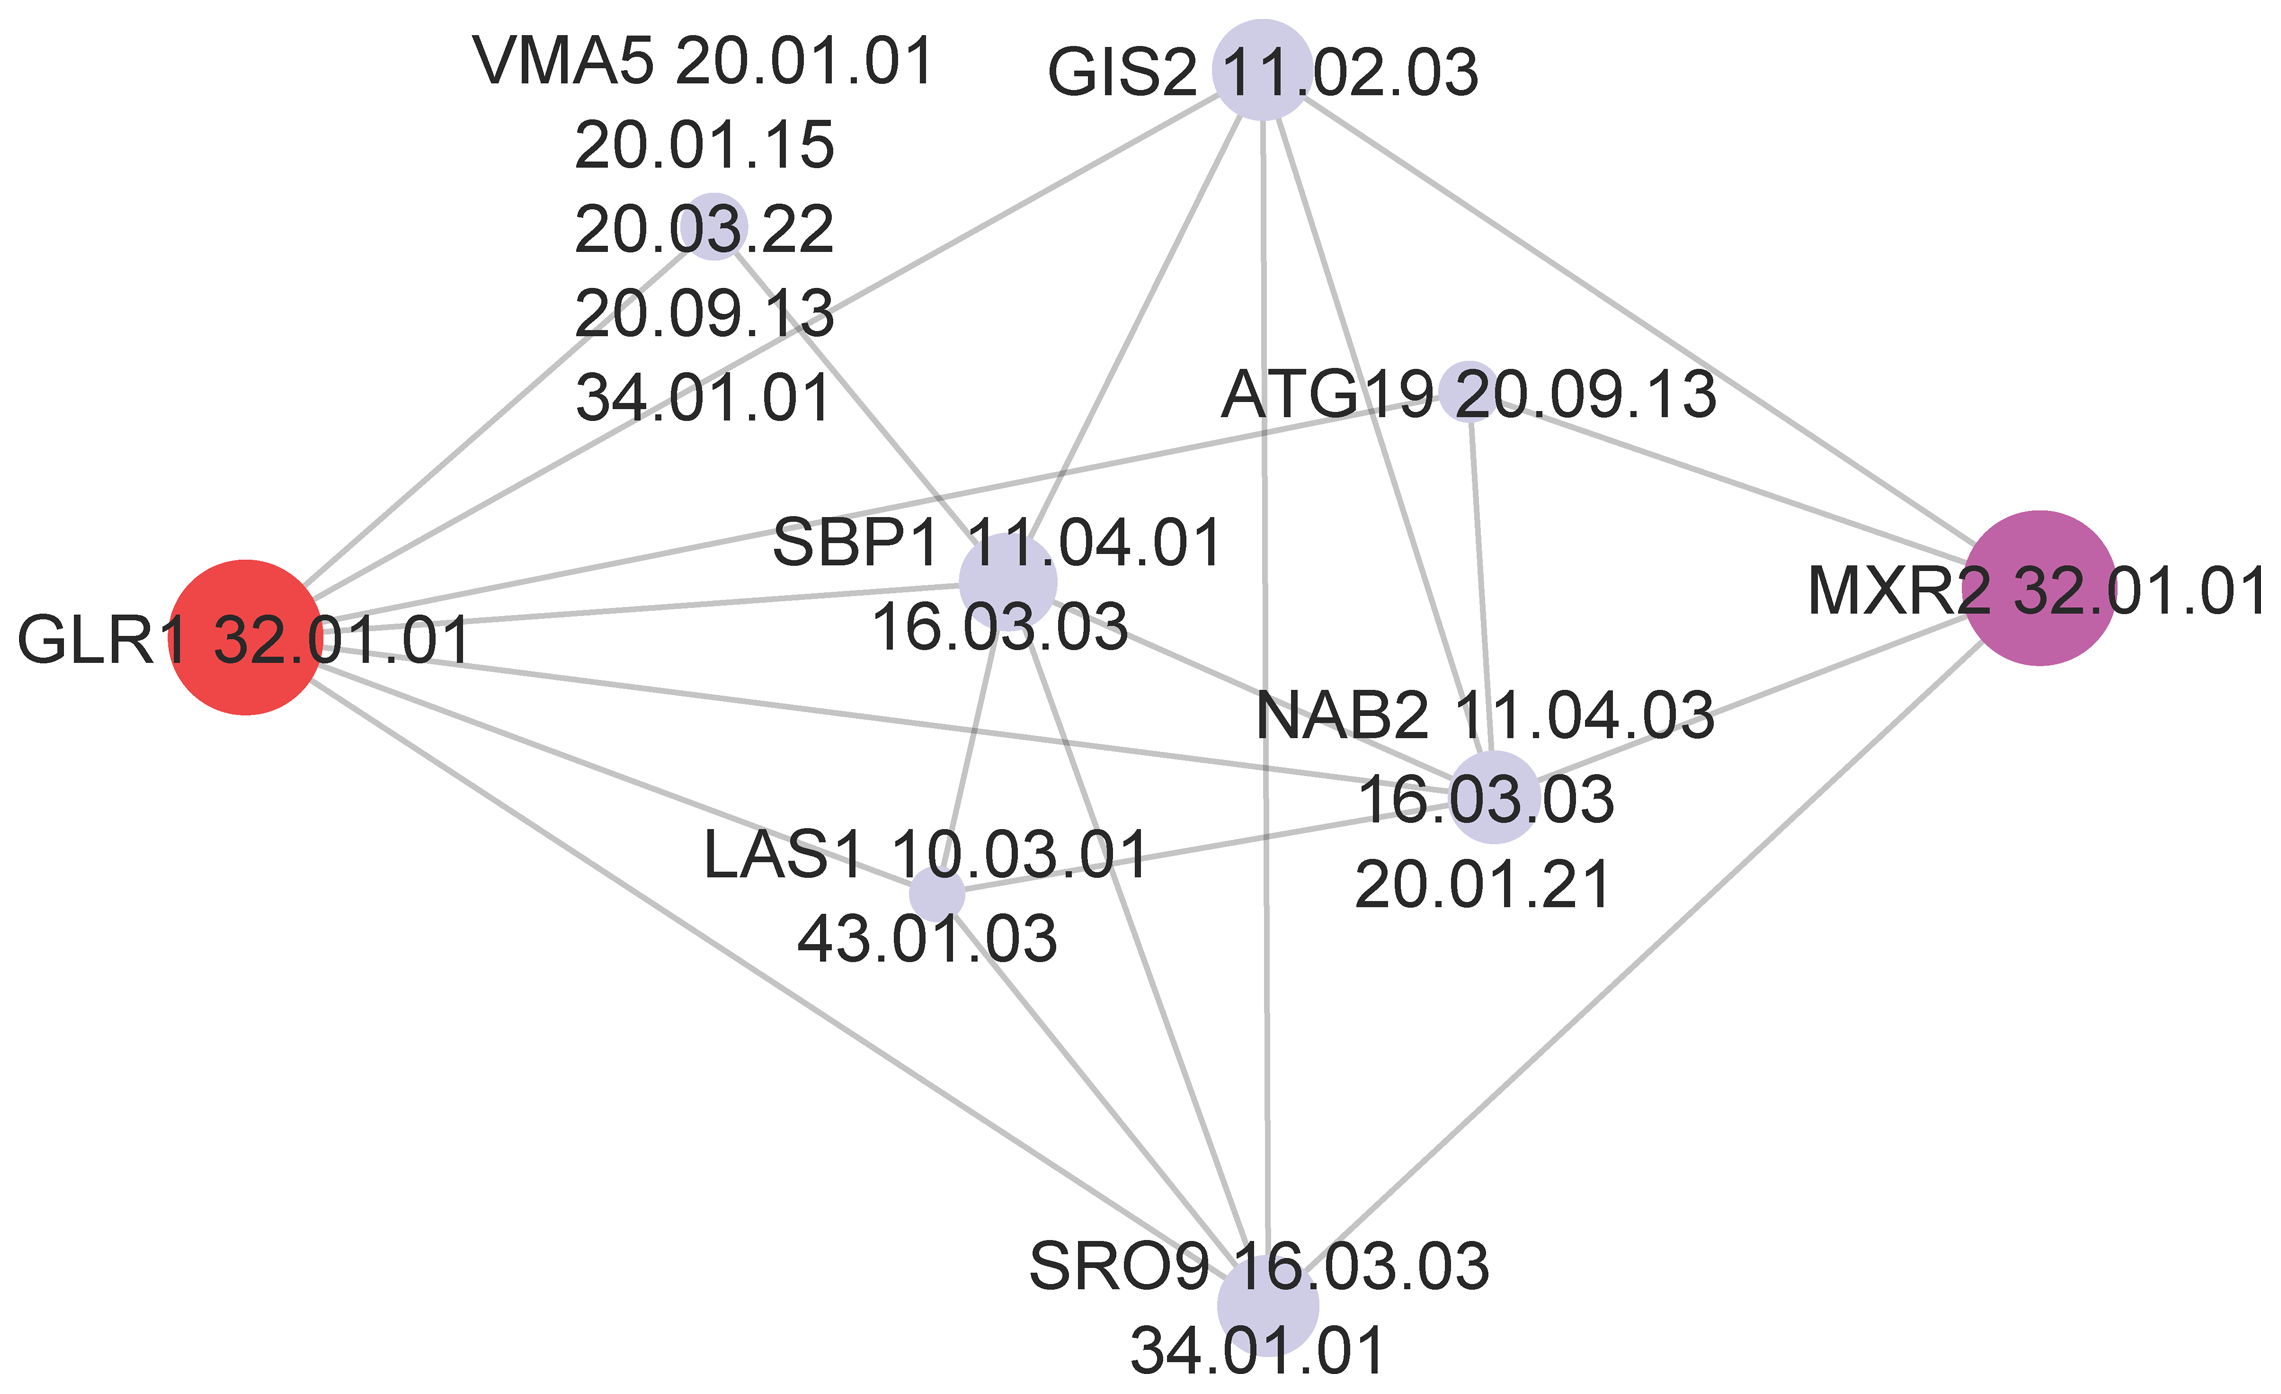
\includegraphics[width=0.75\textwidth]{dsd_ex.png}
\caption{An example of functional annotation with the DSD metric from Cao et al.
~\cite{10.1371/journal.pone.0076339}. It is clear that the vertex colored purple is not a direct
neighbor of the red vertex with respect to the shortest path distance metric. However, the purple
vertex has a DSD distance closest to the red vertex, and they have the same label. Meanwhile, the
direct neighbors of the purple vertex have different labels.}
\label{fig:PPI_example}
\end{figure}

Cao et al. used four different prediction algorithms to compare the effectiveness of the DSD metric
to that of the shortest path metric. Both weighted and unweighted majority voting algorithms, as
well as the $\chi^{2}$ neighborhood algorithm, multi-way cut algorithm, and functional flow
algorithm were used to compare the predictive performance of these metrics. The DSD metric was
expected to perform better that the shortest path metric, since the small characteristic path length
of the PPI network causes the notion of a shortest paths neighborhood to lose significance. All
vertices in this network are close to every other vertex in the graph, so any neighborhood would
contain a large portion of the vertices in the graph.

We used a similar approach in our project, studying the DSD metric and
incorporating it into a label prediction algorithm.

\subsection{Graph model for recommender systems} Huang, Chung, and Chen~\cite{huang2004graph}
introduce a generic graph model for e-commerce transaction data that can support various
recommendation methods. The two-layer graph model proposed represents relationships between products
and customers. In this model, each layer consists of vertices representing products or customers.
Three types of edges in this two layer system capture the inputs to this model from real world data.
Edges between two customers capture similarity based on available demographic data, answers to
questionnaires, and web usage patterns. Edges between two products capture similarity using
descriptions of the product. Finally, edges between customers and products capture transaction
information such as purchase history, customer rating, and related browsing behavior. Figure
\ref{fig:recommender_example} illustrates an example of the two-layer graph model.

\begin{figure}[h] \centering 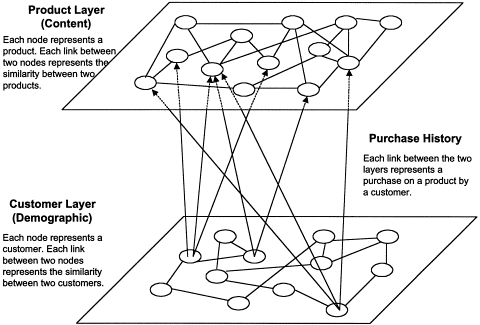
\includegraphics[width=0.75\textwidth]{recommender_ex.png}
\caption{The two-layer graph model proposed by Huang, Chung, and Chen~\cite{huang2004graph}.}
\label{fig:recommender_example}
\end{figure}

Huang, Chung, and Chen considered three different recommendation
methods to use on the model mentioned previously. The direct retrieval method looks at a customer's
previous purchases and products purchased by similar customers to retrieve products to recommend to
the customer. The association mining method uses the purchase history of a customer to generate
association rules about purchasing patterns in order to predict the customer's next purchases. The
high-degree association retrieval method uses weights on edges to represent association strength and
examines paths between the target customer vertex and a product vertex to calculate an association
estimate and determine if the product should be recommended. Transactions from one of the largest
online bookstores in Taiwan were used for data including 9695 books, 2000 customers, and 18,771
transaction records.

The two-layer graph model introduced by Huang, Chung,
and Chen can be interpreted as a graph labeling problem. As a simple example,
we can take the vertices and edges from just the customer layer of the two-layer model. Since the
customer layer included information about demographic data and web usage patterns, we could label
customers with age or certain websites visited and try to predict the labels of prospective
customers. We can perform a similar analysis with the product layer as well as with the whole model
including the interlayer edges.

Such a model can be very useful for advertisers who wish to come up with a
strategic advertising plan. Assuming that an advertisement would have more success if it were shown
to people more likely to buy the product being advertised, we can use the graph model to predict
which customers would buy the product. The product layer can be used to find all products similar to
the product being advertised. Then, we can construct a graph in which vertices are customers who had
bought similar products, and edges existed between customers who had bought the same product. A
prediction algorithm incorporating the DSD could be used to predict the customers who would buy the
product if we knew a few customers that had already bought the product, or were very likely to buy
the product.

Overall, this study shows that subject-knowledge can be used to create real
world graphs (customer layer, product layer, purchase history). We can extend
this to see how subject-knowledge can be used to determine weights during
the voting process for label prediction methods. Labels can also be 
determined from subject-knowledge. However, these labels must have an
underlying structure or intuition behind them in order for label prediction
algorithms to work.


\subsection{Laplacian Eigenmaps} Belkin and Niyogi~\cite{belkin2002laplacian} propose an algorithm
for constructing a locality-preserving representation of data sampled from a low dimensional
manifold embedded in a higher dimensional space. An example can be found in $n\times n$ gray scale
images of a fixed object taken by a moving camera. These images give data points in
$\mathbb{R}^{n^{2}}$, but the inherent dimensionality of this data should be the number of degrees
of freedom of the camera. The presented algorithm constructs a representation of the data that
reduces the dimensionality of the data.

Belkin and Niyogi construct a weighted graph from a given set of points
in $\mathbb{R}^{n}$. Each point is represented by a vertex, and edges are drawn between neighboring
points. Neighborhoods can be determined using $k$ nearest neighbors or $\varepsilon$-neighborhoods.
Weights are determined using heat kernels, or simply adjacency. Finally, eigenmaps are used to
reduce dimensionality of the data.

$1000$ binary $40 \times 40$ images of vertical and horizontal bars at arbitrary points were
randomly chosen as data. The Laplacian Eigenmap algorithm and Principal Component Analysis (PCA) was
applied to this data and compared. The Laplacian Eigenmap algorithm produced a data representation
that clearly showed separate clusters for the vertical and horizontal bars, which PCA failed to do.

This study is quite different from the previous two studies. However, it still raises some interesting questions in relation to our project.
The Laplacian Eigenmaps algorithm focused on being able to detect graph structure, assuming that
the given data lies in a lower dimensional manifold. In our project, we try 
to detecting properties of graph structure that allows prediction methods
using the DSD to perform well. We could also examine whether label prediction
methods using the DSD would be able to detect these lower dimensional manifolds.

